\documentclass{beamer}
\usetheme{default} % Szeged, Singapore, Boadilla, boxes, Pittsburgh
\usepackage{etex}

% BASIC PACKAGES
% Support for Danish characters UTF-8
\usepackage{ucs}
\usepackage[utf8x]{inputenc}

%Enumerate
\usepackage{enumerate}

% English bibliography
\usepackage[english]{babel}

% Coloring of text and tables
\usepackage{color}
\usepackage{colortbl}

% Framed boxes
\usepackage{framed}

% Allow for custom floats
\usepackage{float}

% Landscape environment
%\usepackage{lscape}

% inline lists
\usepackage{paralist}

%For ensuring space after commands
\usepackage{xspace}

% Compact itemize
%\usepackage{mdwlist}

% MATHEMATICS
\usepackage{amsthm}			% AMS theorem package
\usepackage{amsfonts}
\usepackage{amsmath}		% AMS math symbols
%\usepackage{amssymb}		% More symbols!
\usepackage{mathtools}		% Even more symbols!
\usepackage{latexsym}		% Holy shit I can't believe there are still more symbols!
\usepackage{stmaryrd}		% Symbols! When will it end?
%\usepackage{textcomp}		% The unholy God of symbols has spoken. We need more symbols
%\usepackage{gensymb}
\usepackage{bussproofs}		% For making prettier type trees!

%Multiline comments etc..
\usepackage{verbatim} 

%Hopefully give us definitions..
%\input{Definitions.tex}

%Support for figures and various stuff for tables
%\usepackage[pdftex]{graphicx}	% JPEG, PNG
%\usepackage{caption}			% Put captions on everything, including stuff you can't normally do it to (for example subfigures)
\usepackage{wrapfig}			% Stuff for wrap figs
\usepackage{subfig}				% insert several subfigures in a figure
\usepackage{flafter}			% prevents floats from appearing before their definiton
\usepackage{sidecap}			% Allows text next to image
\usepackage{array}				% Used with tables - give the ability to align text to center or bottom of cell.
\usepackage{multirow}			% Used to create multi column and multi row spanning cells.
\usepackage{multicol}			% Same as multirow, but for columns. (This package may be redundant)
\usepackage{longtable}			% Tables split over several pages
\usepackage{slashbox}			% Slashed cells, eg. boxes that are split diagonally
%Path for images, images are in image/, compiled images are in bin/images/
\graphicspath{{bin/images/}}
%Allow LaTeX to accept images with dot in the filename
\usepackage{grffile}

% tikz
%\usepackage[version=0.96]{pgf}
%\usepackage{tikz}
%
\usetikzlibrary{petri,arrows,shapes,backgrounds,automata,positioning,fit}
\tikzstyle{arc}=[->,>=stealth,thick]
\tikzstyle{transportArc}=[->,>=diamond,thick]
\tikzstyle{inhibArc}=[->,>=o,thick]
\tikzstyle{every place}=[circle,thick,draw=black!75,fill=black!10,minimum size=6mm]
\tikzstyle{every transition}=[thick,draw=black,fill=black!75,minimum width=2mm,minimum height=5mm]
\tikzstyle{every token}=[fill=black,text=black]
\tikzstyle{dots}=[circle,text=black,minimum size=6mm]
\newcommand{\tzbox}[2]{\matrix(#1){#2\\}; }




\usepackage{pgfplots}
\pgfplotsset{width=5cm}

% Conditionals nice
\usepackage{ifthen}

% Really, really slack formatting
% This relaxes what is considered "bad" formatting,
% and should suppress warnings ala "underfull \hbox" and the like
\tolerance=10000            % Knuth-infinite
\hbadness=10000
\emergencystretch=1.5em     % EMERGENCY STETCH
\hfuzz 10000pt
\widowpenalty=10000
\vfuzz \hfuzz
\raggedbottom

%See http://www.eng.cam.ac.uk/help/tpl/textprocessing/squeeze.html
\setlength{\intextsep}{1.5ex}

% Different font in captions
\newcommand{\captionfonts}{\small}

\makeatletter  % Allow the use of @ in command names
\long\def\@makecaption#1#2{%
  \vskip\abovecaptionskip
  \sbox\@tempboxa{{\captionfonts #1: #2}}%
  \ifdim \wd\@tempboxa >\hsize
    {\captionfonts #1: #2\par}
  \else
    \hbox to\hsize{\hfil\box\@tempboxa\hfil}%
  \fi
  \vskip\belowcaptionskip}
\makeatother   % Cancel the effect of \makeatletter

% ALGORITHMS%
%\usepackage{algorithmic}
\usepackage[ruled]{algorithm}
\usepackage{algpseudocode}
%Algorithmic should use "Input:" and "Output:" instead of "require:" and "ensure:"
\algrenewcommand{\algorithmicrequire}{\textbf{Input:}}
\algrenewcommand{\algorithmicensure}{\textbf{Output:}}

\beamertemplatenavigationsymbolsempty

% CUSTOM MACROS
\newcommand{\tech}{GreenFlow\xspace}
\newcommand{\phase}{\ensuremath{p}\xspace}
\newcommand{\fcirc}{\ensuremath{circ_{future}}\xspace}
\newcommand{\ti}{\ensuremath{t}\xspace}
\newcommand{\tslow}{\ensuremath{\ti_{r}}\xspace}
\newcommand{\tgreen}{\ensuremath{\ti_{g}}\xspace}
\newcommand{\dist}{\ensuremath{d}\xspace}
\newcommand{\vel}{\ensuremath{v}\xspace}
\newcommand{\velmax}{\ensuremath{v_{max}}\xspace}

% METADATA
\author{Karsten Jakobsen og Sabrine Mouritsen \\\vspace{1mm}\textit{Kandidatstuderende i datalogi ved Aalborg Universitet}}
\title{GreenFlow: Reducering af br\ae ndsstofforbug\\ved hastighedstilpasning til trafiklys}
\pagenumbering{arabic}
\date{28. januar 2013}

\setbeamertemplate{footline}[page number]


\begin{document}
\begin{frame}[plain]
  \titlepage
\end{frame}

\AtBeginSection[]{
	\frame<beamer>{ 
		\frametitle{Oversigt}   
		\tableofcontents[currentsection,subsections] 
 	}
}

\begin{frame}{Oversigt}
\pdfbookmark[0]{Contents}{toc}
\setcounter{tocdepth}{1}
\tableofcontents
\setcounter{tocdepth}{2}
\end{frame}


%%%%%%%%%% DO NOT EDIT BELOW, THIS WILL BE AUTO GENERATED %%%%%%%%%%
\section{Introduction}

%motivation
It is well known that a vehicle driving at a constant velocity use less fuel than an accelerating vehicle due to the physical laws of motion.
%The physical laws of motion say that an accelerating vehicle consumes more fuel than a vehicle driving at a constant velocity.\cite{Vejdir}
In order to save fuel, one should therefore try to drive with a constant speed. 
However, several factors hinders drivers in driving at a constant velocity. 
These factors are for example merging roads, blocking vehicles, traffic incidents and traffic lights. 
It is esimated that 1.8 bilion danish kroner is lost on fuel each year on vehicles stopping for traffic light signals in Denmark \cite{Vejdir}.

%the problem of traffic lights
Traffic lights hinders the flow of traffic as it blocks vehicles arriving from one direction in order to allow other vehicles to drive through the intersection.
Each direction of the intersection is given a time period in which vehicles are allowed to pass through the intersection. 
Normally, a driver will only be able to guess when the light is going to change based on local knowledge of the area. 

Looking at Figure \ref{fig:Introduction:network} vehicle $\veh_2$ is approacing the intersection.
%If he have spottet a red light for some time, it is likly that the signals are going to change soon. He can either, take the chance and keep driving at the same speed, until the last momment where he need to brake. Or he can slow down and limp toward the intersection and then maybe avoid a full stop at the traffic light. 
Now assume that vehicle $\veh_2$ knows the distance $\dist_3$ where he has to stop for the traffic light. 
Then also assume that vehicle $\veh_2$ knows that in at least $4$ seconds the traffic ligth will change to green. 
Then it is posible to calculate a speed for vehicle $\veh_2$ such that it will drive the distance $\dist_3$ in at least $4$ seconds. 
Now by the time the vehicle reaches the intersection the signal will have changed and a full stop is avoided.
\begin{figure}[htb]
\centering
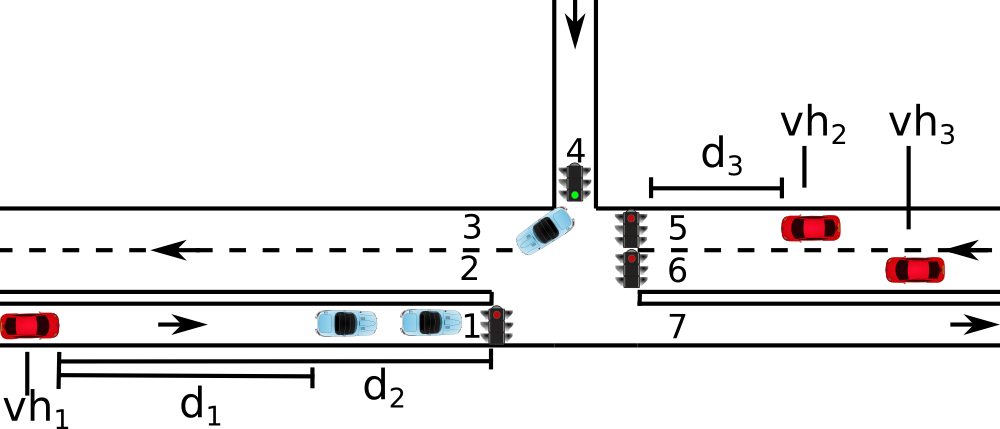
\includegraphics[width=0.5\textwidth]{images/introNetwork.png}
\caption{Eksample network}
\label{fig:Introduction:network}
\end{figure}

Road authorities try to design traffic light signals such that the flow of traffic is maximised in all directions.
This can be very difficult, especially in junctions with changing traffic density through out the day.
Two main techinques are used in traffic lights: pretimed traffic controllers, where the signals loop between red, yellow and green in a predefined pattern; and traffic actuated controllers, where approacing vehicles are detected by road-side detectors such that the signals can be adjusted to the current traffic flow. 
The cost of upgrading a traffic light with detectors is 200.000-300.000 danish kroner, not counting extra maintenance costs to repair broken detectors\cite{Vejdir}.

The focus of this article is to investigate whether it is possible to reduce fuel consumption at traffic ligths by matching the speed to the traffic lights. 
We investigate this through simulations with real world map data, traffic data and traffic light programs, both with crossing traffic and road-side senors. %TODO check we do this
We use the traffic simulator SUMO (Simulation of Urban Mobility)\cite{sumo} interfaced via TraCI (Traffic Control Interface)\cite{traci} which is a full scall microscopic traffic simulator.
The system that we propose, is designed with the assumption that very few vehicle will be using it initialy. 
Because of this, we cannot rely on communication between vehicles.
We also assume that traffic lights and vehicles can communicate such that the phases of the traffic lights are avaiable.
We assume the vehicles use a GPS system that handels the communication and that provides a route to travers.
We do not require any further equipment that this.
Additionally, we assume that all drivers follow the rules of traffic, e.g. dives below the speed limit, do not drive into other vehicles, wait for crossing traffic.

%TODO: outline of the article
//Outline of the article


%Modern traffic lights have sensors known as \textit{induction loops} that can detect vehicles driving on the roads.
%These sensors are used to regulate the signals in relation to the number of vehicles approaching the intersection \cite{Vejdir}. %TODO do we need this?
%If it is possible to reduce the stop-and-go behaviour at traffic lights, it might be possible to reduce the fuel consumption.
%section describing terms of traffic traffic light phase, cycle time ect


%model discribing what we do

%section describing problem with sensors \TODO do we need this?
%A traffic light using only a timer to regulate the traffic is relatively easy to predict if the phases and cycle time is known. 
%However, when we introduce induction loops that are are effected by vehicles ariving in an unpredicteble pattern, then the traffic light will also to some extent become unpredicteble. 








\section{Related Work}\label{sec:RelatedWork}
%TODO: Rearrange this section

The main purpose of our work is to help drivers reduce their fuel consumption by adjusting driving speed to traffic lights.

%TODO: 
% SignalGuru
% http://www.audi.com/com/brand/en/tools/news/pool/2010/06/audi_travolution_.html
% TRANSYT

SignalGURU\cite{SignalGURU} is a similar project 


The authors of \cite{VANETsim} have proposed an idea similar to ours, in that they evaluate whether drivers should accelerate or decelerate when approaching a traffic light.
They also use the simulator SUMO to simulate their methods. 
Contrary to our approach, they rely on communication between nearby vehicles to estimate the number of blocking vehicles such that they can calculate the exact distance.
Their road network is very simple, and do not include any crossing traffic or road senors, and their results are therefore based on a very simplified environment. 
The network that we use is a replica of an often used road in Aalborg, Denmark. 
This one and a half kilometer section of Aalborg includes both traffic lights, crossing traffic, road sensors, and we model it using real observed dimensions, traffic light phases and congestion levels.

One method for designing traffic lights has been proposed in \cite{SOTL} that ensures green waves based on wireless communication between vehicles and traffic lights. 
Their results show a decrease in waiting time by 50 \% in their comparisons. 
Waiting time is the difference between the actual travel time and the minimal travel time (deviding the allowed speed with the travel distance).
The authors of \cite{ITLC} also propose a mehtod for adjusting the traffic lights to the traffic. 
They use reinforcement learning and a voting system amongst vehicles at or near a traffic light to calculate the total gain of different light settings. 
Their results show a reduction in congestion and in some cases they reduce the waiting time by more that 25 \%.

Another related issue is to re-route vehicles in order to avoid congestion. 
This way, drivers will be able to drive more smoothly an hence reduce their fuel consumption. 
Three strategies for re-routing vehicles to avoid congestion has been proposed in \cite{congestionAvoidance}. 
They collect real-time data on the congestion levels from both vehicles and road-side sensors, and provide individual re-routing strategies to the drivers based on the results. 
Through simulations they show that the travel time is 104 \% longer with no re-routing than their best result.

%Simulators
Simulations are a widely used technique for testing hypothesis in the traffic worlds.
Several types of simulation algorithms exist including macroscopic, mesoscopic, microscopic and hybrids.
Macroscopic algorithms model the flow of traffic abstracting the individual vehicles away, whereas mesoscopic models the vehicles but still at an abstract level. 
Microscopic algorithms models vehicles and their behaviour in detail which allows a much more detailed analysis \cite{meso-micro}. 
Hybrid algorithms can be any combination of the aforementioned.
Two major microscopic traffic simulators of today are SUMO (Simulation of Urban Mobility)\cite{sumo} and VISSIM (VISSIM: A microscopic Simulation Tool to Evaluate Actuated Signal Control including Bus Priority)\cite{vissim}.
Both are microscopic simulators, which we will need in order to model for exampel turn lanes.
VISSIM is a comercial tool whereas SUMO is an open source project.
We will be using SUMO when evaluating \tech.

%Several methods for modeling the movement of vehicles also exist.  %TODO: Need cites
%Amongst these are Monte Carlo models \cite{} that use random data, car following models \cite{} where cars follow leading cars, automatas where vehicles follow deterministc rules \cite{} and much more.








\section{Model}\label{sec:Model}
In this section we describe the model that is used to find the speed that will let a vehicle arraive at the next traffic light as it turns green.
See Figure~\ref{fig:Introduction:network} for references.

\subsection{Vehicles}
A vehicle, $\veh$, is an entity that moves along a route.
Each vehicle has an identifier, $\vehid$, a constant acceleration, $\vehacc$ and deceleration, $\vehdec$ and a current position, \vehpos. 
The position is either an edge or a connection (see Section~\ref{sec:map}).
The position is updated as the vehicle moves.
For simplicity we do not consider different drivering behaviours, and operate with one type of vehicle. 

\subsection{Map}\label{sec:map}
A map is a directed graph, $G = (V, E, C)$ where $V$ is a set of vertices, $E$ is a set of edges representing road segments and $C$ is a set of connections between edges.
An egde represents one direction of a road segment.
Every edge $\edge\in E$ has a starting point $\estart\in V$, an end point $\eend\in V$ and a maximum speed $\espeed\in\mathbb{R}$. 
The lenght of an edge is the euclidean distance between $\estart$ and \eend denoted as \elength.
In Figure~\ref{fig:Introduction:network} we have five egdes: two to the west of traffic light, two to the east and one to the north.

By connecting edges through connections, it is possible to model exactly the possible paths through a junction - for example disallowing a right turn.
A connection is also associated a traffic light phase, $\cphase$ detailing when this connection has a red, green or yellow signal (see Section~\ref{sec:phases}).
A juction is therefore made up of several connections that connect the road segments that one can drive to and from.
For example each possible legal pass through the intersection in Figure~\ref{fig:Introduction:network} is a connection as shown in Figure~\ref{fig:Model:Connection} as red arrows. 
A connection, $\con$ is hence unidirectional from one vertex, $\cestart\in V$ to another vertex, $\ceend \in V$, and a connection is made for each lane of the edges.
The example in Figure~\ref{fig:Introduction:network} hence have six connections assuming one cannot make U-turns.
Connections can be seen as a type of edge associated with a phase.
With this abstraction, it is possible to use standard route computing algorithms such as Dikstra's algorithm or A*.

\begin{figure}[h]
\centering
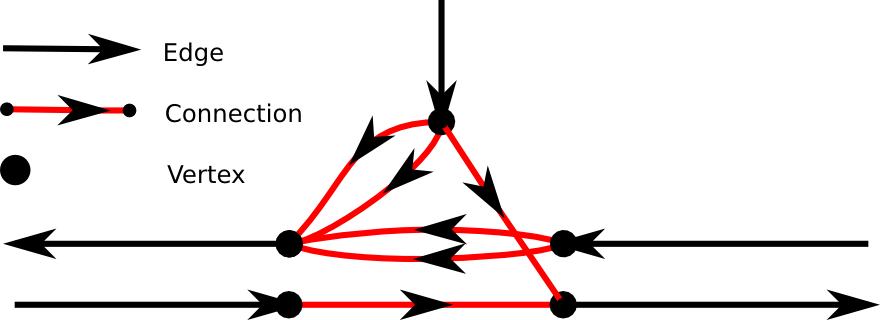
\includegraphics[width=0.4\textwidth]{../images/ConnectionNetwork.png}
\caption{Connection network of Figure \ref{fig:Introduction:network}}
\label{fig:Model:Connection}
\end{figure}

\subsection{Traffic Light Phases}\label{sec:phases}
Each connection in a traffic light has a phase that details the light setting for just this one connection.
SUMO limits the allowed light settings to $red$, $yellow$ and $green$.
A phase of a traffic light, $\phase$ is defined as $\langle(\light_0, \ti_0),(\light_1, \ti_1),\dots, (\light_n, \ti_n) \rangle$ where $t_i>0$ and the light setting is $\light_i\in \{red, yellow, green\}$ in $\ti_i$ seconds for $0 \leq i \leq n$.
There must exist at least one occurence where $\light_i = green$ for $i \in \{0 \dots n\}$. 
A connection in an unregulated junction will simply have the phase $\langle(green, \infty)\rangle$.
Let $\Ccirc{\phase} = \sum_{i=0}^{n}\ti_i$ be the circulation time of \phase where $(\light_i, \ti_i)\in \phase$, and $|\phase|=n$.
A typical circulation time of a phase is between $35$ to $80$ seconds but can up to $110$ seconds. 
The yellow periodes are often $4s$ before a red periode and $2s$ before a green period\cite{vejtrafik}.

\subsection{Junction}
We define a junction \ju to be a set of connections, $\jucons \subseteq C$. 
A junction can be either regulated or unregulated. 
In an unregulated traffic light traffic must give way to traffic coming from the right. 
In a regulated traffic light vehicles will have to check the phase $\cphase$ of the connection \vehpos. 
A junction is said to be unregulated iff $\forall c \in \jucons | \cphase = \langle(green, \infty)\rangle$

\subsection{Routes}
A route, $\route$, is a sequence of edges on the map, $\langle \edge_0, \edge_1, \dots \edge_n \rangle$, where $\exists \con$ such that $\eendi{i} = \cestart$ and $\estarti{i+1} = \ceend$ for $0\leq i< n$.
The vehicle starts at $\edge_0$ and moves along the sequence until $\edge_n$ has been reached.






\section{Mathematics}

\subsection{Without acceleration or deceleration}
Calculating the needed speed, $h$, when acceleration and deceleration is not taking into consideration, for arriving at the next traffic light while it is green.
We use the standard formula for calculating velocity and calculate two velocities: one for arriving at the traffic light just as it changes to green and one when it chances to red. The desired velocity is therefore somewhere in between.
\[h_g = \frac{s}{t_g}\]
\[h_r = \frac{s}{t_r}\]

\[h_r \leq h \leq h_g\]

where
\begin{itemize}
\item $s$ is the distanced between the vehicle and the traffic light
\item $t_g$ is the number of seconds before the traffic light changes to green
\item $t_g$ is the number of seconds before the traffic light changes to red
\item $h_g$ is the speed one needs to drive in order to arrive at the traffic light when it changes to green
\item $h_g$ is the speed one need to drive in order to arrive at the traffic light when it changes to red
\item $h$ is the recommened speed
\end{itemize}

\section{Test Results}\label{sec:Test}
In this section, we verify that simualations give useful results, and evaluate to what extend \tech improve traffic flow and reduce fuel consumption.

\subsection{Verification of the Simulator}
It is imporant to verify that the results obtained from the simulator actually matches the real-world observations.
We compare the results from the simulator with GPS trajectories collected in the project "Spar P\aa\ Farten".
If the results are similar, we may deduce that the simulator provides usable results.
We compare the simulator with the GPS data on three fronts: 
\begin{enumerate*}
\item Comparison based on a metric based on average speed, number of stops and waiting time
\item Comparison of the travel distance 
\item Comparison of the driving speed
\end{enumerate*}

We only look at data from the main road of Hobrovej in the northern direction, only use GPS trajectories between 10 am and 2 pm on weekdays, and use a spawning rate of $0.8$ vehicle per second.
Tests show that this give comparable data.

\subsubsection{Validation Metric}
The validation metric is based on three key measurements: speed, waiting time and number of stops. 
Waiting time is the difference between the travel time and free flow time, which is how long it will take to drive the same distance driving at the speed limit and never stopping.
The free flow time is $93s$.
We say a vehicle has stop when its speed drops below $10km/s$, and say that it move again when it drives faster than $15km/h$.%TODO: Check
The average value for all vehicles on the main road of Hobrovej togeather with the population standard deviation (STDEV) can be seen in Table~\ref{table.valMetric}.
The difference between simulated and GPS data are minimal indicating that SUMO simulates these factors satisfactory.
The deviation is quite large for waiting time and number of stops.
The is, however, expected as there is a large difference between those that drive through all junctions without stopping, and those that have to stop every time.
\begin{table}
\centering
\begin{tabular}{|l|c|c|c|c|}\hline
 						&  \multicolumn{2}{c|}{SUMO} & \multicolumn{2}{c|}{GPS} \\\hline
 						& Value & STDEV & Value & STDEV \\\hline
Avg. speed ($km/h$) 	& 37.45 & 7.86 	& 35.03 & 6.28 \\\hline
Avg. waiting time ($s$) & 66.90 & 33.97 & 70.35 & 33.07 \\\hline
Avg. number of stops 	& 1.91 	& 0.66 	& 1.80 	& 1.08 \\\hline
\end{tabular}
\caption{Validation metric}\label{table.valMetric}
\end{table}

\subsubsection{Travel Distance}
Travel distance of the real data is plotted in Figure~\ref{fig:TestResults:realDistance} as a function over time. 
We see that the curves flatens at about 300 $m$, 600 $m$, 900 $m$ and 1200 $m$, indicating that the vehicles are stationary at these points.
This corresponds well with the dimensions of Hobrovej and match the four regulated traffic lights.
\begin{figure}[htb]
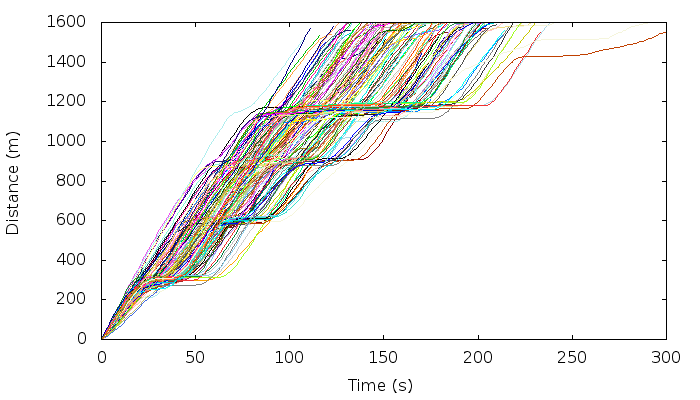
\includegraphics[width=0.45\textwidth]{../images/Real/RealDistance.png}
\caption{Travel distance for real GPS trajectories}
\label{fig:TestResults:realDistance}
\end{figure}

Figure~\ref{fig:TestResults:distance0} also plots the travel distance as a function over time, only for the results of the simulator.
We see that the simulation resembles the real-world results, however, the simulated vehicles tend to hold longer at the traffic lights. 
This is because the phases of traffic lights of the simulation are too different compared to real traffic lights. 
Besides that, the acceleration profiles look similar, and the map has the correct dimensions.%TODO: Det her er uklart

\begin{figure}[htb]
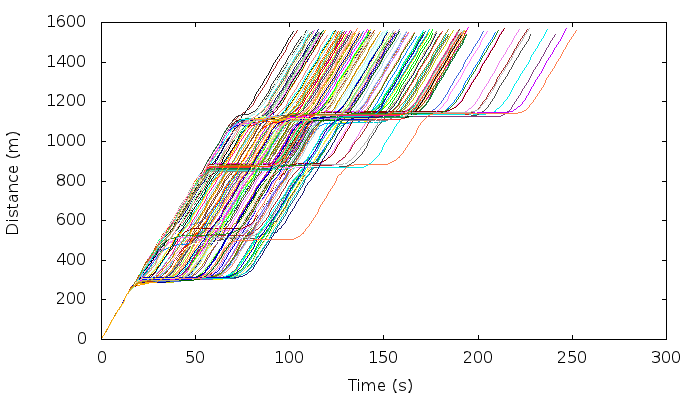
\includegraphics[width=0.45\textwidth]{../images/tp0c0_8/distanceUncontrolled0.png}
\caption{Travel distance for simulated data without \tech}
\label{fig:TestResults:distance0}
\end{figure}

\subsubsection{Driving Speed}
The driving speed as a function over time for the GPS trajectories is plotted in Figure~\ref{fig:TestResults:RealSpeed}.
In order to read the data, only random 20 trajectories have been plotted in this graph.
First of all, we see that most drivers drive at around $50 km/h$, and some drives above the speed limit of $60 km/h$. 
We also see that many drop to around $0 km/h$ and that some are able to avoid a full stop.

\begin{figure}[htb]
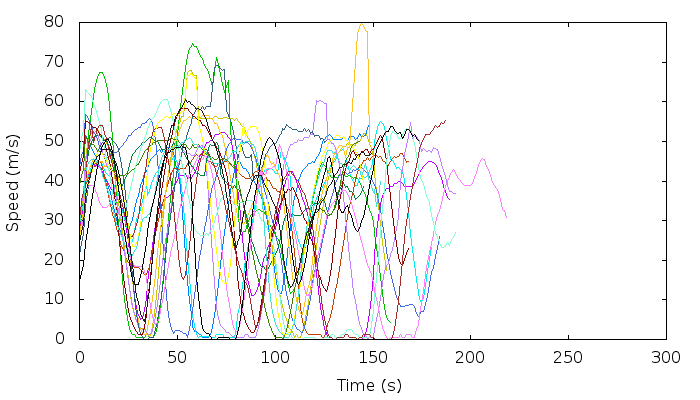
\includegraphics[width=0.45\textwidth]{../images/Real/RealSpeed.png}
\caption{Speed for real GPS trajectories}
\label{fig:TestResults:RealSpeed}
\end{figure}

Plots of the driving speed for the simulated vehicles can be seen in Figure~\ref{fig:TestResults:speed0} as a function over time.
The behaviour of these simulated vehicles are much different from the real drivers.
The simulated drivers almost always either accelerate to the maximum speed or decelerate to $0 km/h$. 
A few decelerates to $40 km/h$, but that is most likely because the traffic light turns green just before they arrive.
No one breaks the speed limit.
The simulated vehicles therefore have a much more aggresive driving behaviour than what we see in the real-world data.
This will also mean that they use more fuel than a real driver would use. %TODO: Kristian har en eller anden kommentar. Kan ikke helt læse det, måske "How know?"
However, we see that the metric values for the real and simulated data are not that different.

\begin{figure}[htb]
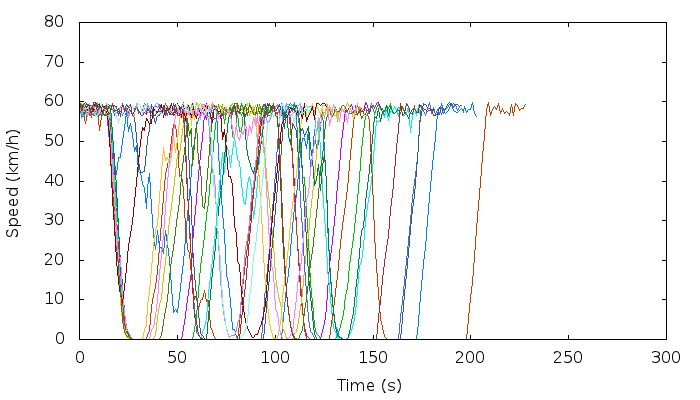
\includegraphics[width=0.45\textwidth]{../images/tp0c0_8/speedUncontrolled0.png}
\caption{Speed for simulated data without \tech}
\label{fig:TestResults:speed0}
\end{figure}

\begin{table}
\centering
\begin{tabular}{|l|l|cc|cc|}\hline
Percent using 			& With/w.o. & \multicolumn{2}{c|}{Fuel} 	& \multicolumn{2}{c|}{Time}\\
\tech					&\tech		& $ml$		& Diff.			&	$s$	& Diff.\\\hline
\multirow{1}{*}{0\%}	& Without	&	125.8	&	0\%			&	139 & 0\%		\\\hline
\multirow{2}{*}{10\%}	& With 		&	88.7	&	29.5\%		&	136 & 2.5\%		\\
						& Without 	&	125.3	&	0.4\%		&	135 & 2.9\%		\\\hline
\multirow{2}{*}{50\%}	& With		&	88.1	&	30.0\%		&	131 & 5.8\%		\\
						& Without	&	121.8	&	3.2\%		&	127 & 8.6\%		\\\hline
\multirow{1}{*}{100\%}	& With		&	86.8	&	31.0\%		&	121 & 12.9\%	\\\hline
\end{tabular}
\caption{Average values from the simulations. Diff. is the difference compared to 0 \% using \tech}
\label{tb:TestResults:total}
\end{table}

\subsection{Fuel Consumption}
Reducing the fuel consumption at least for the vehicles using the system is one of the objectives.
No real data on the fuel consumption is aviable to us, and we therefore only compare the simulation with itself. 
Tabel~\ref{tb:TestResults:total} lists the average fuel consumption and travel time for all vehiclees in the network. 
The value "Diff." is the difference to 0 \% using \tech.

Figure~\ref{fig:TestResults:fuelTotal} plots the fuel consumption for all vehicles in the network for two different simulations: one where no vehicles use \tech (blue) and one where all vehicles are using \tech (green).
The number of vehicles are the same in both simulations, and they drive the same routes with the same departure times. 
The only difference is whether they use \tech or not.

The average fuel consumption when all vehicles use \tech is about $86.8 ml$ and about $125 ml$ when no one use \tech.
We therefore see a significant overall reduction in fuel consumption on 31 \% in this setting if \tech is used by everybody.
Looking at just the selected route through the network, we see the same tendency (see Figure~\ref{fig:TestResults:fuelRoute}). 
The average fuel consumption with \tech is about $115 ml$ and about $159 ml$ without, resulting in a reduction of about 28 \%.
%TODO: Consider using 10% in stead of 100% in the two figures below.
\begin{figure}[htb]
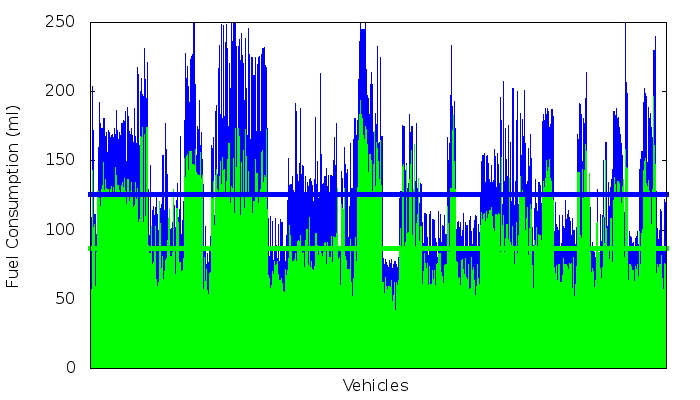
\includegraphics[width=0.45\textwidth]{../images/tp0c0_8/fuelTotal.png}
\caption{Fuel consumption for all vehicles in the network. Blue: 100\% using \tech, green: 0\% using \tech}
\label{fig:TestResults:fuelTotal}
\end{figure}

\begin{figure}[htb]
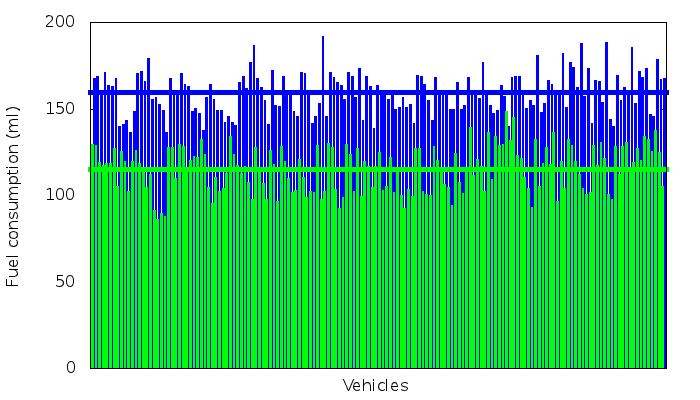
\includegraphics[width=0.45\textwidth]{../images/tp0c0_8/fuelRoute.png}
\caption{Fuel consumption for all vehicles on the selected route}
\label{fig:TestResults:fuelRoute}
\end{figure}

It is, however, more interesting to investigate the influence \tech has when only a few drivers use it.
Figure~\ref{fig:TestResults:combinedFuel} shows the average fuel consumption for four different penetration rates (0 \%, 10 \%, 50 \% and 100 \%) on the main route.
The blue columns show the average fuel consumption for those not using \tech, and the green columns show the average fuel consumption for those using \tech.
The left- and rightmost columns hence show the same average levels as in Figure~\ref{fig:TestResults:fuelRoute}.
When \tech is used in 10 \% of the vehicles, we see a small decrease in fuel consumption for those not using it, and a significant reduction for those using \tech.
The reduction is about 29 \% (reduced to $ml$).
When the penetration rate increases to 50 \%, we again see that the fuel consumption decreases slightly for those not using \tech, but see that it increases slightly for those using it.
This is most likely because vehicles start platooning (driving in groups), where vehicles using \tech force other vehicles to drive slower and the recommended speed may match the traffic lights less when the vehicles huddle together.

\begin{figure}[htb]
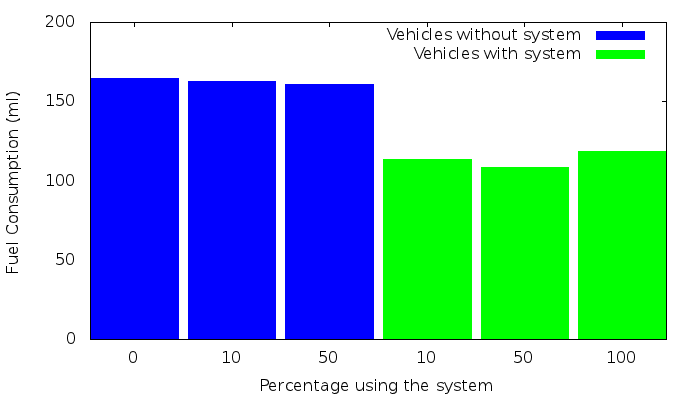
\includegraphics[width=0.45\textwidth]{../images/tp0c1_0/combinedFuel.png}
\caption{Fuel consumption for different penetration rates on the main route}
\label{fig:TestResults:combinedFuel}
\end{figure}

We see this fuel reduction because the vehicles accelerate less rapidly. 
Figure~\ref{fig:TestResults:distance100} shows the travel distance as a function over time when all vehicles use \tech, and Figure~\ref{fig:TestResults:speed100} plots the driving speed as a function over time.
We see that the curves are much more smooth than those in Figure~\ref{fig:TestResults:distance0} and~\ref{fig:TestResults:speed0}, because they avoid stopping, and hence has to accelerate less.
Some vehicles still have to stop, partly because it is impossible to drive the distance between the traffic lights in the time left before it turns green, and partly because there are other vehicles blocking their path.

We can therefore conclude that in the tested use case, we see a significate reduction in fuel consumption at about 30 \% even when it is only implemented in a small subset of the vehicles.
Moreover, vehicles using \tech does not have a negative influence on the fuel consumption of the other vehicles.
\begin{figure}[htb]
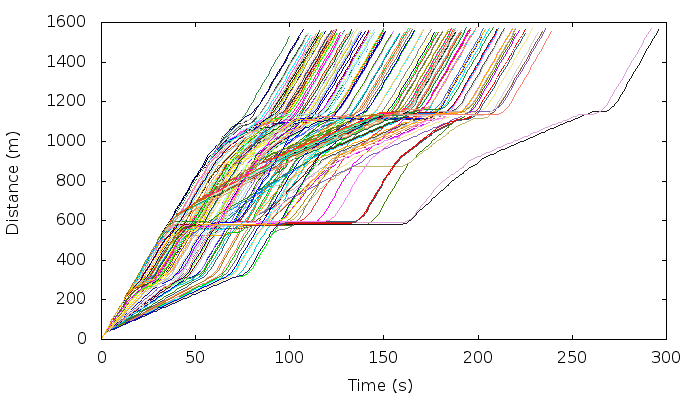
\includegraphics[width=0.45\textwidth]{../images/tp0c0_8/distanceControlled100.png}
\caption{Travel distance for simulated data when 100\% use \tech}
\label{fig:TestResults:distance100}
\end{figure}

\begin{figure}[htb]
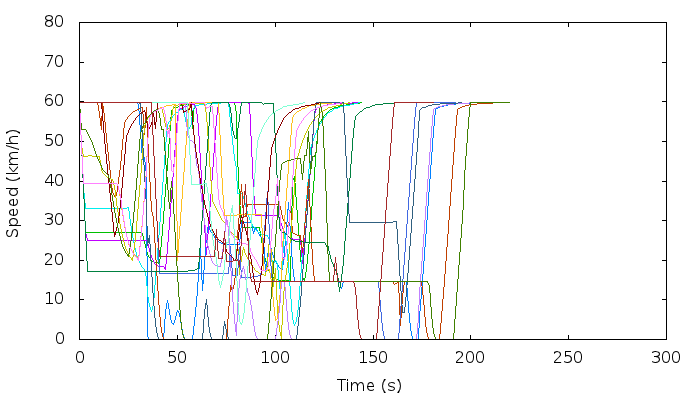
\includegraphics[width=0.45\textwidth]{../images/tp0c0_8/speedControlled100.png}
\caption{Driving speed for simulated data when 100\% use \tech}
\label{fig:TestResults:speed100}
\end{figure}

\subsection{Travel time}
Reducing the fuel consumption is important, but it cannot be at the expense of traffic flow or the vehicles travel time.
Figure~\ref{fig:TestResults:combinedTime} show the average travel time for all vehicles on all routes in the network at different levels of penetration.
With 0 \% using \tech we see an average travel time of $139$ seconds. 
Introducing the systemt to 10 \% of the vehicles reduces this by about 2 \% ($136s$). 
However, as the penetration rate increases, we travel time continues to reduce. 
This is mostly due to the fact that vehicles do not make a full stop at traffic lights, and therefore are able to start faster.

\begin{figure}[htb]
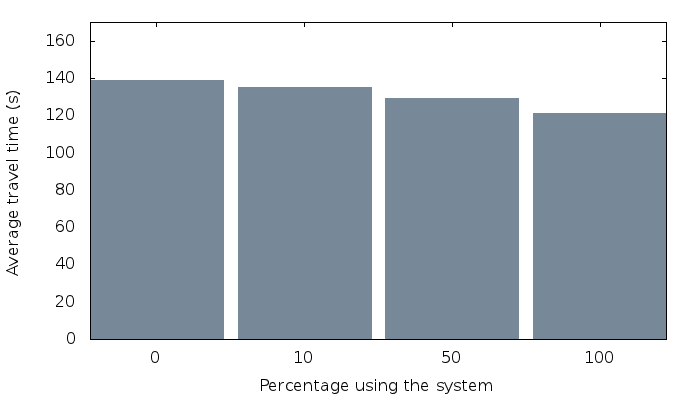
\includegraphics[width=0.45\textwidth]{../images/tp0c0_8/combinedTime.png}
\caption{Travel time for all routes at different level of vehicles using \tech}
\label{fig:TestResults:combinedTime}
\end{figure}

\subsection{Congestion Levels}
%TODO: when does the traffic break? Do we break later than without \tech? Not sure how to read the results. Do not think it looks like we break later.
Normal traffic usualy have peak periods where the traffic is higher than normal \cite{Vejdir}. 
In order to test the effect of the system with different congestion levels we repeated the simulation while changing the rate with which vehicles are spwaning. 
The fuel consumption at different penetration rates (plots) and congestion levels (x-axis) can be seen in Figure \ref{fig:TestResults:congestionFuel}. 
The fuel consumtion does not change much when less than $1$ vehicle spawn per second.
With higher congestion, the traffic seems to break down, most pronouced at lower penetration rates. %TODO: Break down stuff
\begin{figure}[htb]
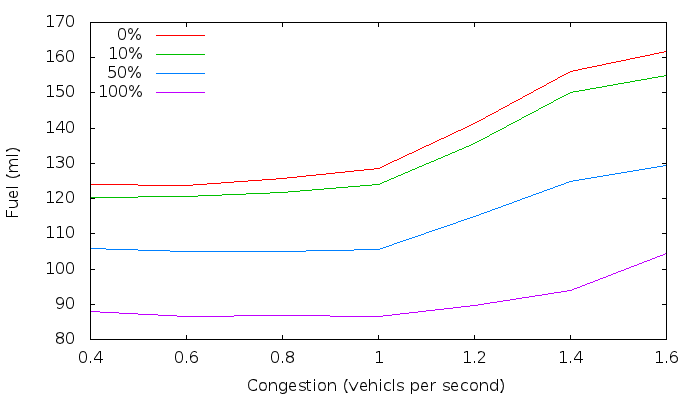
\includegraphics[width=0.45\textwidth]{../images/fuelCongestion.png}
\caption{Fuel consumption at different penetration and congestion levels}
\label{fig:TestResults:congestionFuel}
\end{figure}

In Figure \ref{fig:TestResults:congestionTime} we see the average travel time for all vehicles driving in the simulation compared to the different congestion levels. 
With low congestion there is almost no difference in the travel time.
We clearly see that the travel time increases less when more drivers use \tech as the congestion increases. %TODO: Break down stuff
In a congested network large queues of vehicles build up. 
A large portion of the time a traffic light is green is wasted on the time it takes to get the queue moving. 
A queue of vehicles accelerrating spend less time gaining speed if they are already moving slowly. 
This is likly the reason that the average time of all vehicles improve if enough are using the system.
\begin{figure}[htb]
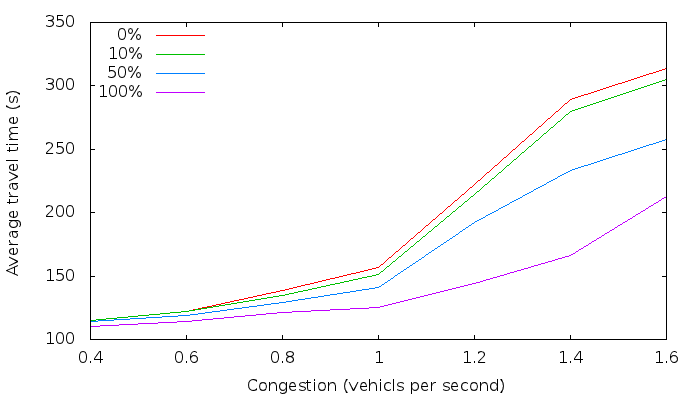
\includegraphics[width=0.45\textwidth]{../images/timeCongestion.png}
\caption{Travel time at different penetration and congestion levels}
\label{fig:TestResults:congestionTime}
\end{figure}

\section{Potential Savings}%TODO: A lot of numbers, how do we make it easier to read? Should it be someting else?
Say that $20,000$ vehicles drive this route a day on average across a year and 78\% drive outside the peak periods, then $15,600$ vehicles can potential benefit from using \tech\cite{}.
$15,600$ vehicles driving without \tech will in a day use $1,965.6 l$ of fuel according to the simulations.
If just 10 \% of these use \tech this is reduced to $1,893.8 l$ where the 10 \% spend $138.84 l$ and the 90 \% use $1,755 l$.
With a liter of fuel costing $12$ DKK the total savings will be $861.12$ DKK a day for this $1.6 km$ section of Hobrovej with 4 regulated junctions.
If there are 222 weekdays in a year, this amounts to about $191,168.64$ DKK.
Imagining that every vehicle on this stretch use \tech, they will in total save $608.4$ $l$ fuel a day, which is $7,300.80$ DDK a day and $1,620,777.60$ DKK a year.
It remains to the investigated what the savings will be on a larger network.







%%%%%%%%%% DO NOT EDIT ABOVE, THIS WILL BE AUTO GENERATED %%%%%%%%%%

\end{document}		